\section{Hacia un Framework para la Comparación de Permisos}
\begin{frame}
 \begin{center}
  \LARGE Framework \\para la \\Comparación de Permisos
 \end{center}
\end{frame}
\begin{frame}
 \frametitle{Hacia un Framework para la Comparación de Permisos}
 \begin{itemize}
  \item Android e iOS permiten cambiar ciertos permisos de una aplicación luego de haberla instalado en el dispositivo.
  \item Es por ello que se ha desarrollado un \textit{framework} para determinar empíricamente el alcance de los sistemas de permisos de ambas plataformas.
 \end{itemize}
 \begin{columns}
  \begin{column}[]{.35\textwidth}
   \begin{exampleblock}{Objetivo I}
    {Se busca dejar en evidencia posibles vulnerabilidades presentes en los modelos de seguridad.}
   \end{exampleblock}
  \end{column}
  \begin{column}[]{.60\textwidth}
   \begin{exampleblock}{Objetivo II}
    {Se pone énfasis en la relación existente entre la privacidad del usuario y el sistema de permisos, analizando cuál es la cobertura del sistema respecto de los datos sensibles para la privacidad.}
   \end{exampleblock}
  \end{column}
 \end{columns}
\end{frame}
\begin{frame}
\frametitle{Hacia un Framework para la Comparación de Permisos}
\begin{columns}
  \begin{column}[]{.60\textwidth}
   \begin{alertblock}{Aplicación Híbrida}
Es una aplicación móvil diseñada en un lenguaje de programación web ya sea HTML5, CSS o JavaScript, junto con un \emph{framework} que permite adaptar la vista web a cualquier vista de un dispositivo móvil.
   \end{alertblock}
  \end{column}
  \begin{column}[]{.35\textwidth}\pause
   \begin{block}{Apache Cordova}
Es un \emph{framework} que permite crear aplicaciones para dispositivos móviles utilizado HTML5, CSS3, y JavaScript, con el objetivo de lograr un desarrollo multiplataforma.
   \end{block}
  \end{column}
 \end{columns}\pause
 \begin{block}{}
El \textit{framework} es \alert{una aplicación móvil híbrida} \pause \structure{desarrollada con Apache Cordova} \pause y está compuesto por varios tests.
 \end{block}\pause
 \begin{block}{}
Cada test pone a prueba a un componente del dispositivo, permitiendo así conocer el alcance de los permisos correspondientes a dicho componente.
 \end{block}
\end{frame}
\begin{frame}
 \frametitle{Hacia un Framework para la Comparación de Permisos}
 \begin{itemize}
  \item Para el presente trabajo se decidió utilizar los emuladores oficiales para testear el \emph{framework} propuesto. \pause
  \item Los emuladores permiten interactuar de la misma manera que se haría con un dispositivo real, pero con el ratón y el teclado, y mediante los botones y los controles del emulador.
 \end{itemize}
\end{frame}
\begin{frame}
 \frametitle{Hacia un Framework para la Comparación de Permisos}
\begin{figure}[hbtp]
    \centering
	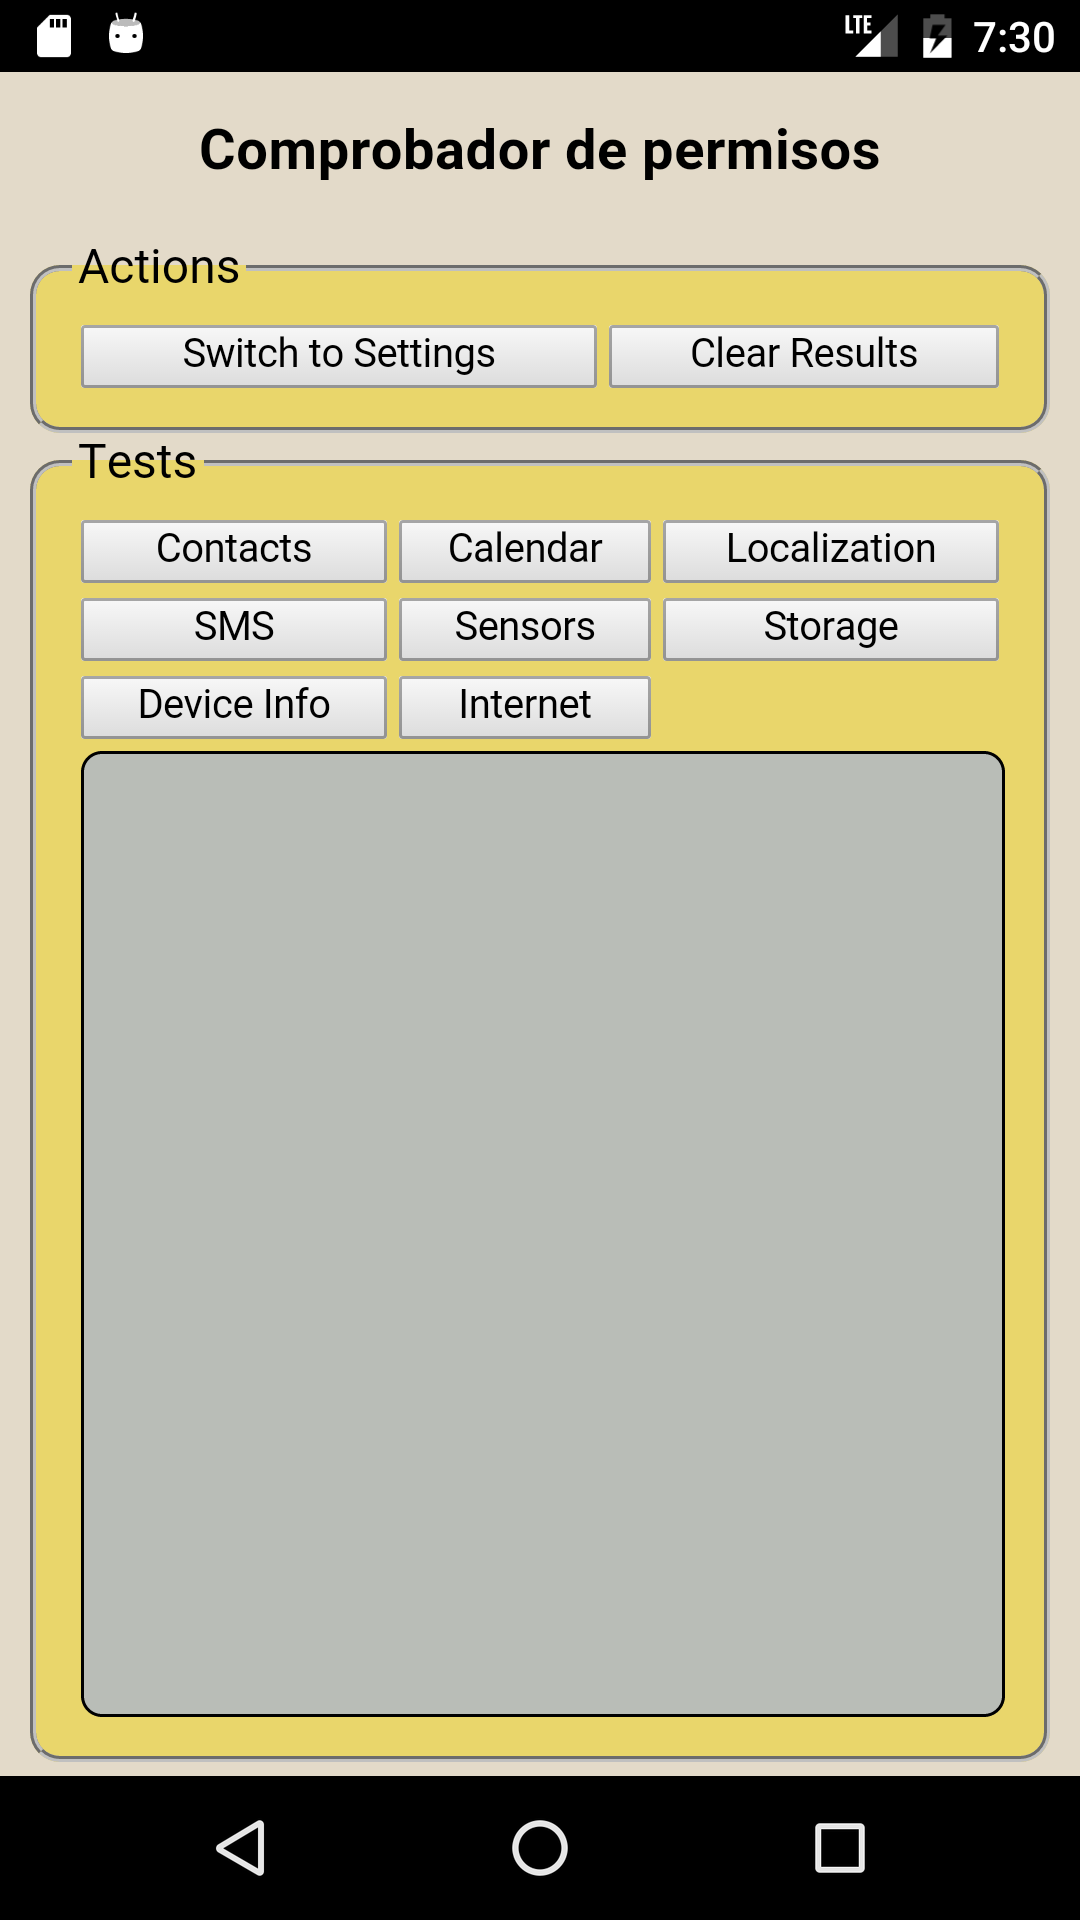
\includegraphics[width=0.3\linewidth]{app_main_view}
	\caption{Áreas del \textit{framework}.}
	\label{fig:chapter05:main_view}
\end{figure}
\end{frame}
\begin{frame}
 \frametitle{Hacia un Framework para la Comparación de Permisos}
 \begin{columns}
  \begin{column}[]{.5\textwidth}
   Utilizando \emph{framework} se pueden testear:
   \begin{itemize}
	\item Contactos
	\item Calendario
	\item Geolocalización
	\item SMS\structure *
	\item Sensores
	\item Almacenamiento
	\item Información del dispositivo
	\item Acceso a Internet
   \end{itemize}
  \end{column}
  \pause
  \begin{column}[]{.5\textwidth}
   Sin embargo, no se pueden testear:
   \begin{itemize}
    \item \alert {WIFI}
    \item \alert {Bluetooth}
    \item \alert {NFC}
    \item \alert {Conexiones USB}
    \item \alert {Micrófono}
    \item \alert {Cámara}
   \end{itemize}
  \end{column}
 \end{columns}
\end{frame}
\begin{frame}
 \frametitle{Hacia un Framework para la Comparación de Permisos}
Para cada uno de los tests se detalla el algoritmo, los plugins de Apache Cordova que se utilizaron para desarrollarlo y una serie de capturas que muestran los casos exitosos y fallidos.\\ \pause
Por ejemplo:
\begin{figure}[hbp]
    \centering
    \begin{subfigure}{0.28\linewidth}
        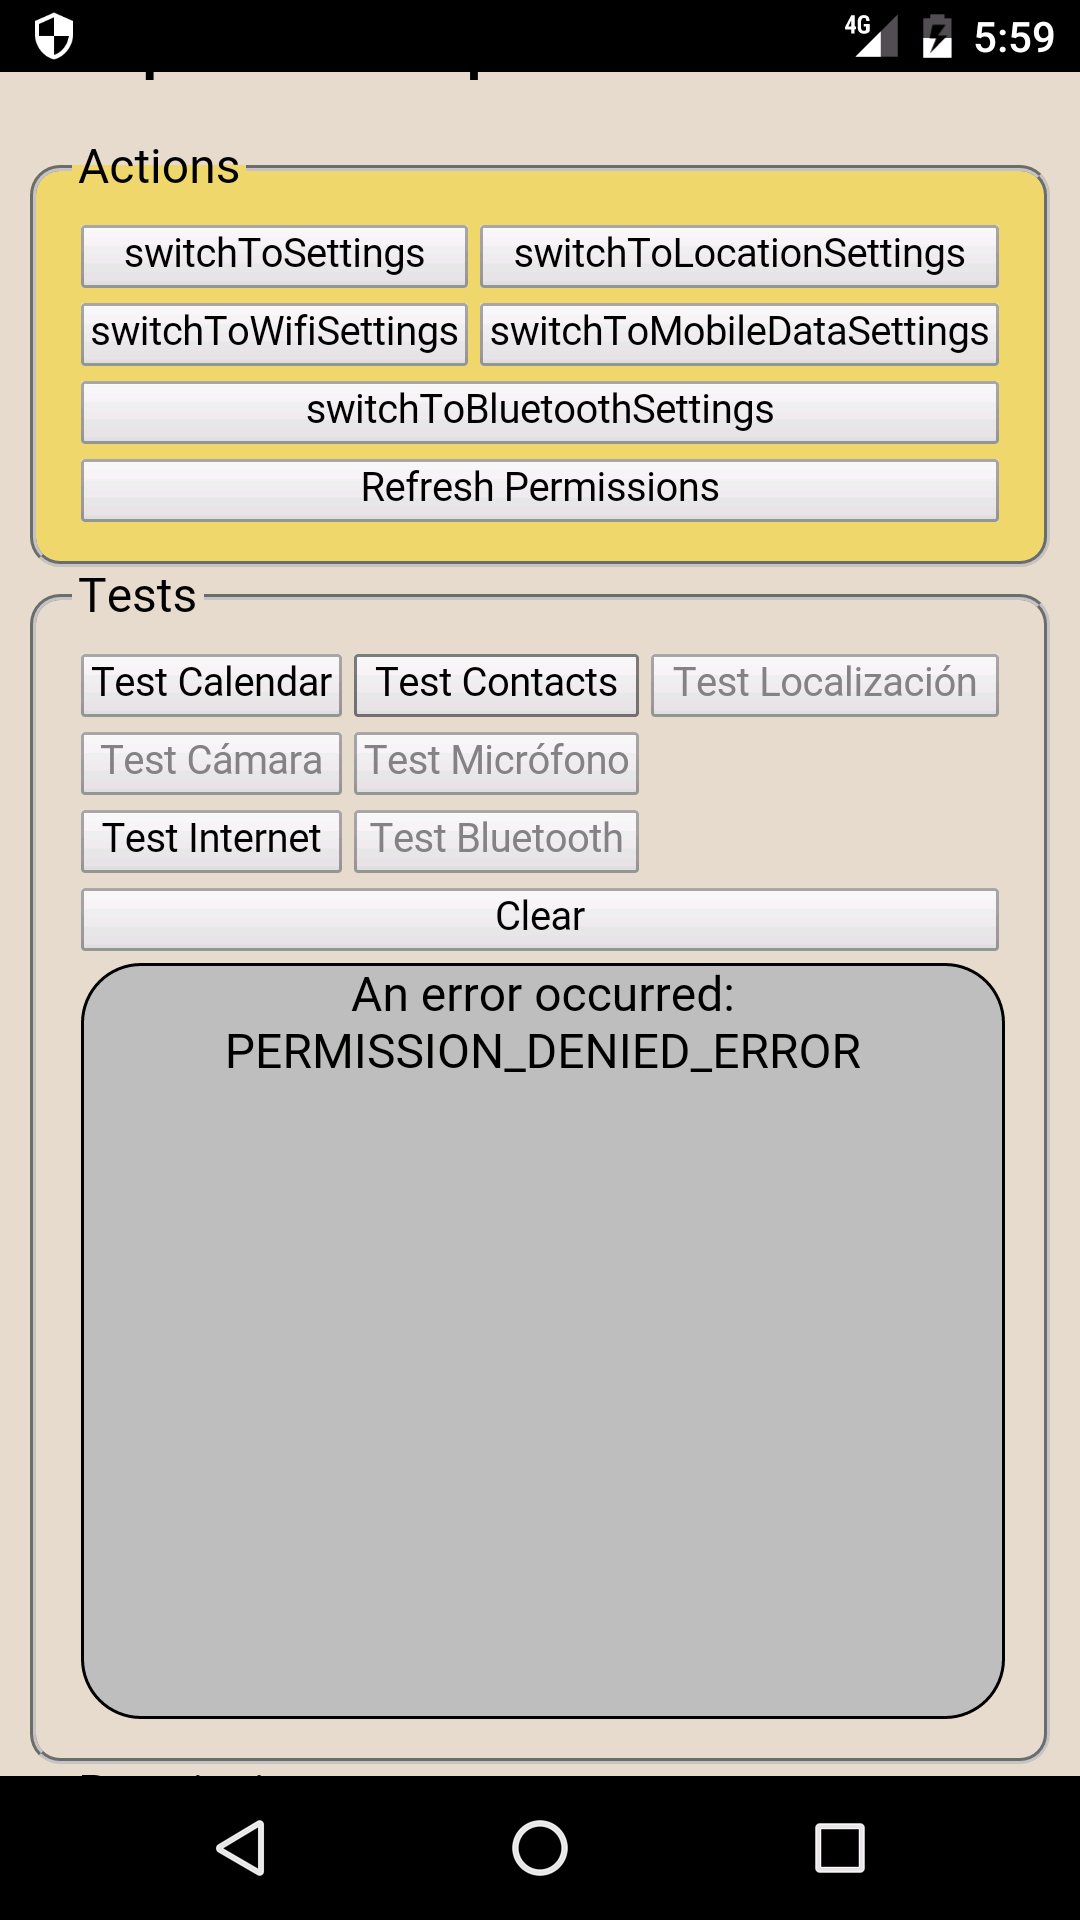
\includegraphics[width=\linewidth]{without_contact}
    \end{subfigure}
    \begin{subfigure}{0.28\linewidth}
        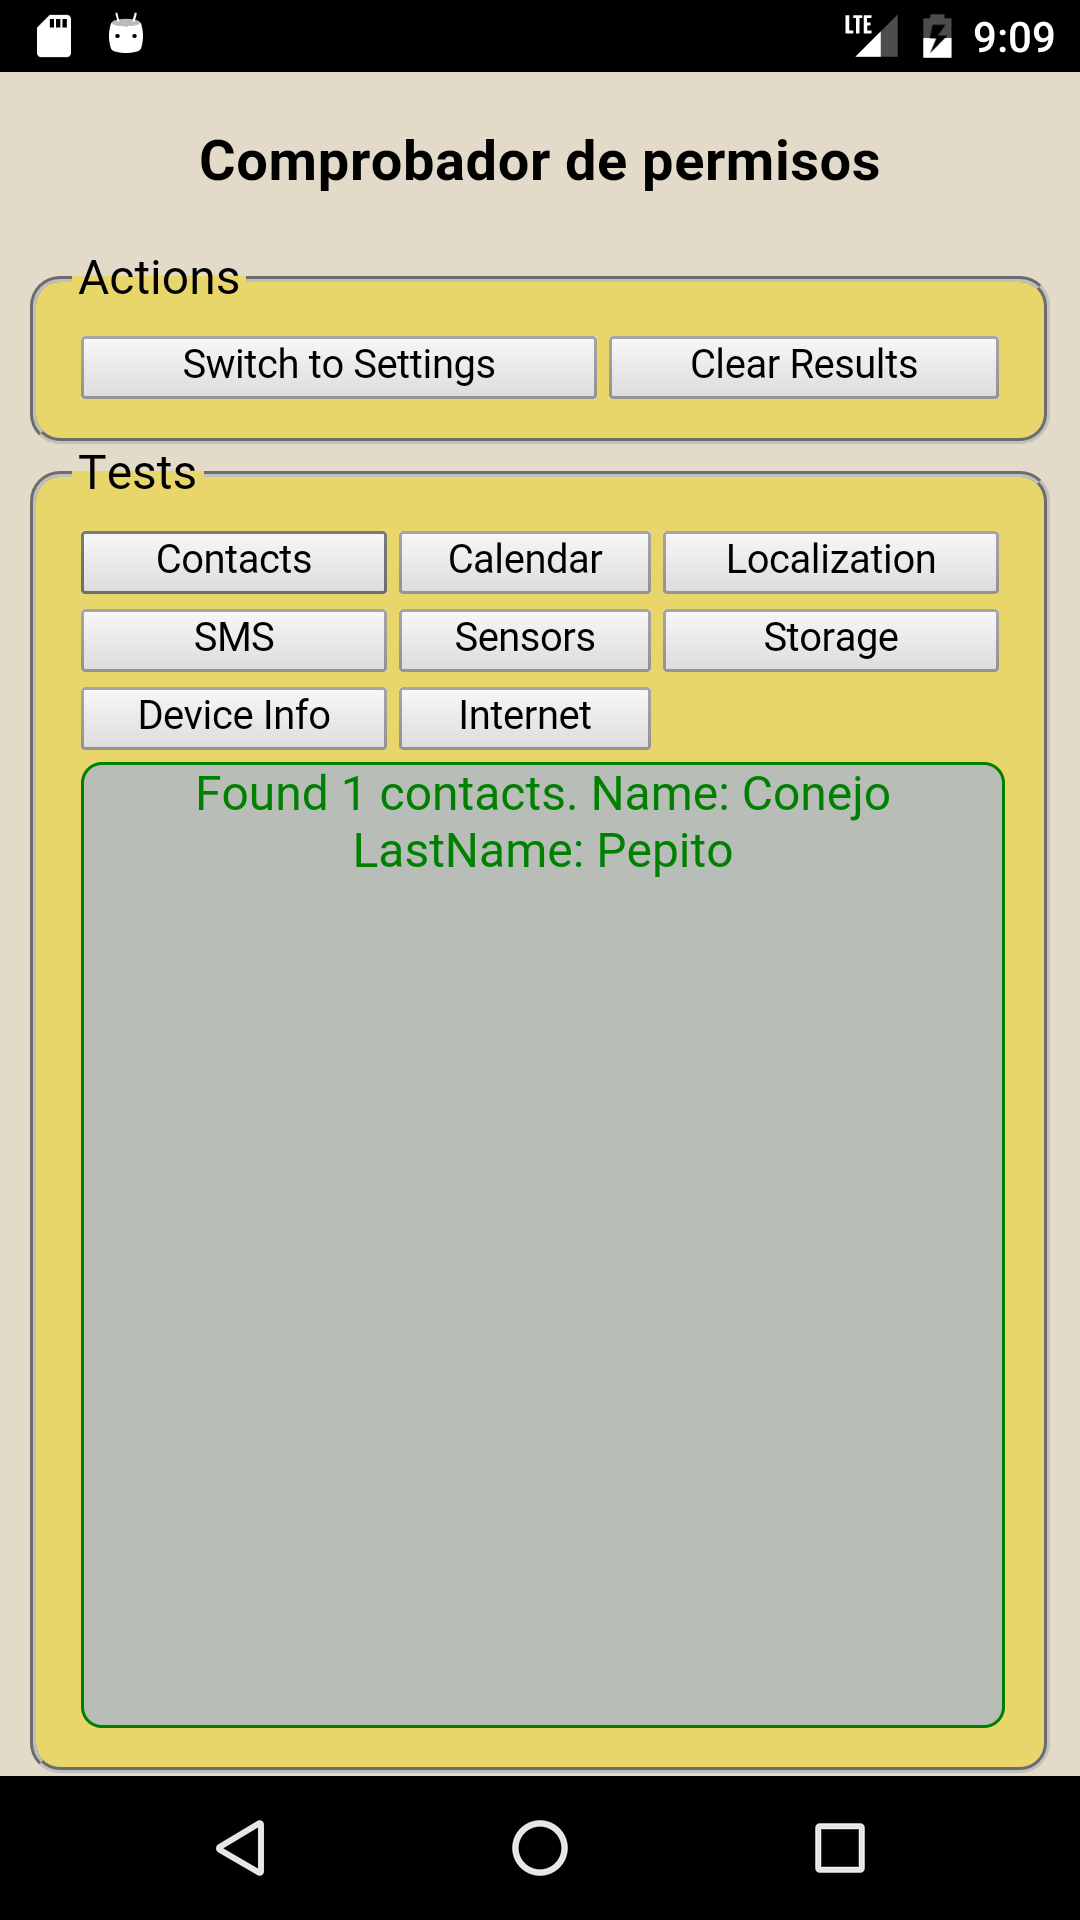
\includegraphics[width=\linewidth]{with_contact}
     \end{subfigure}
	\begin{subfigure}{.40\linewidth}
	\begin{algorithm}[H]
	\algsetup{linenosize=\small}
    \scriptsize
	\begin{algorithmic}[1]
		\STATE Se imprimen por consola todos los contactos.
		\STATE Se crea un nuevo contacto.
		\STATE Se vuelven a imprimir por consola todos los contactos.
	\end{algorithmic}
	\caption{\centering Test de Contactos}
   \end{algorithm}
   \begin{block}{}\tiny
 {Se utilizó el \textit{plugin} \href{https://www.npmjs.com/package/cordova-plugin-contacts}{cordova-plugin-contacts \\(v. 2.3.1)} de Apache Cordova.\\Para correr el test, es necesario tener el permiso \texttt{Contacto}, tanto para Android como para iOS.}
   \end{block}
   \end{subfigure}
    \end{figure}
\end{frame}
\begin{frame}
Luego de correr los tests, se puenden clasificar los componentes testeados en cuatro clases mutuamente excluyentes, según requieran autorización del usuario para utilizarlos. \pause Dichas clases son:
\begin{columns}
  \begin{column}[]{.30\textwidth}
   \begin{tiny}
   \begin{itemize}
    \item \underline{Clase A}: componentes que requieren autorización explícita en ambas plataformas para poder utilizar las funcionalidades que proveen;
    \item \underline{Clase B}: componentes que requieren autorización explícita solamente en Android;
    \item \underline{Clase C}: componentes que requieren autorización explícita solamente en iOS;
    \item \underline{Clase D}: componentes que no requieren autorización explícita para poder utilizar las funcionalidades que proveen.
   \end{itemize}
   \end{tiny}
  \end{column}
  \begin{column}[]{.7\textwidth}
  \begin{table}[H]
    \centering
    \begin{tiny}
	\begin{tabular}{c c c c}
		\hline
		\multicolumn{4}{c}{\emph{\textbf{Permisos}}} \\
		\emph{Clase A} 	& \emph{Clase B}	 & \emph{Clase C}    & \emph{Clase D}\\ \hline \hline
    Contactos    & -    & -    & -\\
    Calendario    & -    & -    & -\\
    Geolocalización    & -    & -    & -\\
    -    & SMS & -    & -\\
    -    & Almacenamiento    & -    & -\\
    -    & -    & -    & Sensores\\
    -    & -    & -    & Información del dispositivo\\
    -    & -    & -    & Acceso a Internet\\ \hline
	\end{tabular}
	\end{tiny}
	\end{table}
  \end{column}
 \end{columns}
\end{frame}